\section{Data Driven Background Estimation Methods}
\label{sec:datadriven}

We have developed two data-driven methods to 
estimate the two potentially dominant backgrounds.
The first method provides an estimate of the number of events with fake leptons (jets misidentified as leptons).
The second method is used to estimate the number of genuine leptons reconstructed with an incorrect charge sign.

\subsection{Data Driven prediction for fake lepton backgrounds}
\label{sec:fakes}

We predict the background from fake leptons using the technique previously implemented in 2010 data analysis
and documented in~\cite{frmethod}.
The idea is to count the number of events for which one lepton passes all final selections and a second lepton
fails the nominal requirements but passes a looser set of requirements. 
We refer to the former lepton as a "numerator" lepton ($n$),
and the latter a "non-numerator" (denominator and not numerator, or $\bar{n}$).
The denominator objects are also referred to as fakeable objects (FO).
The ratio of "numerator" to "denominator" objects is called a "fake rate",
 FR (also known as tight-to-loose ratio, TL).  
A fake rate function is measured in an independent data sample of multijet events.
This fake rate function is measured in bins of lepton $\pt$ and $|\eta |$,
separately for electrons and muons. 

The numerator selections are detailed in Section~\ref{sec:eventsel}. 
The denominator selections are exactly the same as in the inclusive analysis~\cite{ssnote2011}.
They are listed below for completeness.

Muon denominator definition is to relax the following muon requirements from
Section~\ref{sec:eventsel}:
\begin{itemize}
\item $\chi^2$/ndof of global fit $<$ 50 (was $<$ 10);
\item transverse impact parameter with respect to the selected vertex is
$<$ 2 mm (was $<$ 200 $\mu$m);
\item $Iso$ is set to be $Iso < 0.4$  (was $<$ 0.1).
\end{itemize}

Electron denominator definition is to relax the following electron requirements from
Section~\ref{sec:eventsel}:
\begin{itemize}
\item the impact parameter cut is removed (was $<$ 200 $\mu$m);
\item $Iso$ is set to be $Iso < 0.6$ (was $<0.10$).
\end{itemize}

We thus use an extrapolation  in isolation (and impact parameter) to estimate the fake lepton backgrounds 
in both electrons and muons.
This choice of the denominator is designed to be safe determining contributions
from all types of fake lepton candidates arising from jets.
It has already been extensively tested in the inclusive (pre-tagged) same-sign dilepton analysis~\cite{ssnote2011},
where the fake-isolated leptons are expected to be dominated by
heavy flavor jets, in which the lepton candidate is predominantly a real lepton from b/c-quark semileptonic decays.
In this analysis, as discussed in detail below, we find that isolated lepton candidates
not arising from heavy flavor decays have a much larger fraction (dominant for electrons) of all fake leptons.
Closure tests performed on \ttbar\ simulation (still expected to be the dominant source of fakes)
confirm this choice of denominator definition works here as well.

Samples of multijet (inclusive QCD) events in data are selected among events with a single lepton trigger present.
The same requirements are applied to select the multijet-dominated events as in the inclusive analysis~\cite{ssnote2011}.

We repeat all relevant studies performed with 2011 data, as documented in Ref.~\cite{ssnote2011}.
These include 
\begin{itemize}
\item extraction of the fake rates in simulation and data;
\item measurement of the fake-rate dependence on the {\em opposite-side} jet \pt,
	as a measure of the dependence on the progenitor parton momentum in data;
\item closure tests on \ttbar\ after the baseline and search region selections.
\end{itemize}
Results of other tests performed in Refs.~\cite{ssnote2011,frmethod} apply here in part,
with the main caveat that they are the most relevant for fakes not from 
the heavy flavor as well:
\begin{itemize}
\item closure tests in W+jets and double-fake in QCD MC samples 
	(even though none of these are expected to contribute significantly even at the baseline
	selection level);
\item estimates of the residual W+jet and Z contamination in the sample;
\item comparison with the fake rate measured in events with enhanced heavy flavor
	contribution using b-tagging (the variation observed here is up to about 20\% for electrons and
	muons in both simulation and data and are fractionally much less important
	here).
\end{itemize}
We arrive to essentially the same conclusions on the performance of the fake-rate method
as we did in the past.
In particular, we find that the method works reasonably well, still with a systematic
uncertainty of about 50\%.
In the following we summarize the measurement of the fake rate and provide several highlights
of the studies with the current dataset.

The nominal fake rates are measured requiring an "opposite side" jet with $\pt>40~\GeV$, 
separated by $\Delta R > 1.0$ from the FO.
The electron fake rates are measured separately for triggers with an isolation requirement and
for triggers without any isolation requirement on the electron.
Results of the measurement are summarized in Table~\ref{tab:frelectronTCaloIso} for triggers
with calorimeter isolation (as used for $e\mu$ events), and in Table~\ref{tab:frelectronTCaloIsoTrkIso} 
for triggers with both the calorimeter and tracker isolation requirements (as used for $ee$ events).
Results for electron triggers without an isolation requirement are provided in Table~\ref{tab:frelectronTNoIso}
as a reference.
The muon fake rates are measured using all single-muon triggers described in Ref.~\cite{ssnote2011}.
The measurement is summarized in Table~\ref{tab:frmuon}.

\begin{table}[htb]
\begin{center}
\begin{tabular}{c|ccccc}
\hline
\backslashbox{$|\eta|$}{$p_T$} & 10.000 -- 15.000 & 15.000 -- 20.000 & 20.000 -- 25.000 & 25.000 -- 35.000 & 35.000 -- 55.000 \\ \hline\hline
0.000 -- 1.000 & 0.2773 $\pm$ 0.0072 & 0.1784 $\pm$ 0.0072 & 0.1759 $\pm$ 0.0079 & 0.1789 $\pm$ 0.0084 & 0.2583 $\pm$ 0.0148 \\ \hline
1.000 -- 1.479 & 0.2749 $\pm$ 0.0121 & 0.2177 $\pm$ 0.0132 & 0.1977 $\pm$ 0.0115 & 0.1924 $\pm$ 0.0117 & 0.3026 $\pm$ 0.0197 \\ \hline
1.479 -- 2.000 & 0.2415 $\pm$ 0.0152 & 0.1806 $\pm$ 0.0137 & 0.1871 $\pm$ 0.0099 & 0.1916 $\pm$ 0.0095 & 0.2379 $\pm$ 0.0135 \\ \hline
2.000 -- 2.500 & 0.2827 $\pm$ 0.0146 & 0.2607 $\pm$ 0.0156 & 0.2420 $\pm$ 0.0119 & 0.2561 $\pm$ 0.0116 & 0.3225 $\pm$ 0.0154 \\ \hline
\end{tabular}
\caption{\label{tab:frelectronTCaloIso}Electron fake rate measured in bins of the electron candidate \pt\ and $\eta$
for electrons collected using triggers with a calorimeter isolation requirement.}
\end{center}
\end{table}

\begin{table}[htb]
\begin{center}
\begin{tabular}{c|ccccc}
\hline
\backslashbox{$|\eta|$}{$p_T$} & 10.000 -- 15.000 & 15.000 -- 20.000 & 20.000 -- 25.000 & 25.000 -- 35.000 & 35.000 -- 55.000 \\ \hline\hline
0.000 -- 1.000 & 0.3783 $\pm$ 0.0218 & 0.2932 $\pm$ 0.0279 & 0.2365 $\pm$ 0.0298 & 0.2713 $\pm$ 0.0324 & 0.3690 $\pm$ 0.0527 \\ \hline
1.000 -- 1.479 & 0.3556 $\pm$ 0.0357 & 0.3617 $\pm$ 0.0496 & 0.2364 $\pm$ 0.0405 & 0.2353 $\pm$ 0.0460 & 0.4667 $\pm$ 0.0644 \\ \hline
1.479 -- 2.000 & 0.2326 $\pm$ 0.0372 & 0.1638 $\pm$ 0.0344 & 0.2000 $\pm$ 0.0332 & 0.2260 $\pm$ 0.0314 & 0.2793 $\pm$ 0.0426 \\ \hline
2.000 -- 2.500 & 0.3357 $\pm$ 0.0399 & 0.2736 $\pm$ 0.0433 & 0.2362 $\pm$ 0.0377 & 0.2681 $\pm$ 0.0377 & 0.3645 $\pm$ 0.0465 \\ \hline
\end{tabular}
\caption{\label{tab:frelectronTCaloIsoTrkIso}Electron fake rate measured in bins of the electron candidate \pt\ and $\eta$
for electrons collected using triggers with calorimeter and tracker isolation requirements.}
\end{center}
\end{table}

\begin{table}[h]
\begin{center}
\begin{tabular}{c|ccccc}
\hline
\backslashbox{$|\eta|$}{$p_T$} & 10.000 -- 15.000 & 15.000 -- 20.000 & 20.000 -- 25.000 & 25.000 -- 35.000 & 35.000 -- 55.000 \\ \hline\hline
0.000 -- 1.000 & 0.1985 $\pm$ 0.0141 & 0.1535 $\pm$ 0.0177 & 0.1260 $\pm$ 0.0212 & 0.1567 $\pm$ 0.0247 & 0.2198 $\pm$ 0.0434 \\ \hline
1.000 -- 1.479 & 0.1951 $\pm$ 0.0253 & 0.1867 $\pm$ 0.0318 & 0.1870 $\pm$ 0.0352 & 0.1800 $\pm$ 0.0384 & 0.3333 $\pm$ 0.0624 \\ \hline
1.479 -- 2.000 & 0.1880 $\pm$ 0.0339 & 0.1696 $\pm$ 0.0355 & 0.1481 $\pm$ 0.0279 & 0.1548 $\pm$ 0.0279 & 0.2596 $\pm$ 0.0430 \\ \hline
2.000 -- 2.500 & 0.2583 $\pm$ 0.0356 & 0.3084 $\pm$ 0.0446 & 0.1797 $\pm$ 0.0339 & 0.2836 $\pm$ 0.0389 & 0.3191 $\pm$ 0.0481 \\ \hline
\end{tabular}
\caption{\label{tab:frelectronTNoIso}Electron fake rate measured in bins of the electron candidate \pt\ and $\eta$
for electrons collected using triggers without isolation requirements.}
\end{center}
\end{table}

\begin{table}[htb]
\begin{center}
\begin{tabular}{c|ccccc}
\hline
\backslashbox{$|\eta|$}{$p_T$} & 5.000 -- 10.000 & 10.000 -- 15.000 & 15.000 -- 20.000 & 20.000 -- 25.000 & 25.000 -- 35.000 \\ \hline\hline
0.000 -- 1.000 & 0.2760 $\pm$ 0.0028 & 0.2127 $\pm$ 0.0024 & 0.1808 $\pm$ 0.0032 & 0.1541 $\pm$ 0.0043 & 0.1441 $\pm$ 0.0009 \\ \hline
1.000 -- 1.479 & 0.3119 $\pm$ 0.0042 & 0.2527 $\pm$ 0.0036 & 0.2100 $\pm$ 0.0048 & 0.1820 $\pm$ 0.0067 & 0.1770 $\pm$ 0.0015 \\ \hline
1.479 -- 2.000 & 0.3340 $\pm$ 0.0042 & 0.2694 $\pm$ 0.0037 & 0.2238 $\pm$ 0.0049 & 0.2197 $\pm$ 0.0072 & 0.2018 $\pm$ 0.0016 \\ \hline
2.000 -- 2.500 & 0.3343 $\pm$ 0.0061 & 0.2741 $\pm$ 0.0054 & 0.2174 $\pm$ 0.0071 & 0.2012 $\pm$ 0.0108 & 0.2150 $\pm$ 0.0027 \\ \hline
\end{tabular}
\caption{\label{tab:frmuon}Muon fake rate measured in bins of the muon candidate \pt\ and $\eta$.
The uncertainties are statistical only.}
\end{center}
\end{table}

Figures~\ref{fig:frmuon}  and~\ref{fig:frelectron}  show the projection on $\pt$ and $|\eta|$ of these fake rates
for electrons and muons, respectively.
Electron fake rates measured for triggers with an isolation requirement are slightly higher than those
for triggers without an isolation requirement, as expected.
The difference, even though it's not very large, is significant enough and we treat fake rates for these triggers
separately.
The dependence of the fake rates on the away-jet momentum is also shown on these figures.

\begin{figure}[h]
\begin{center}
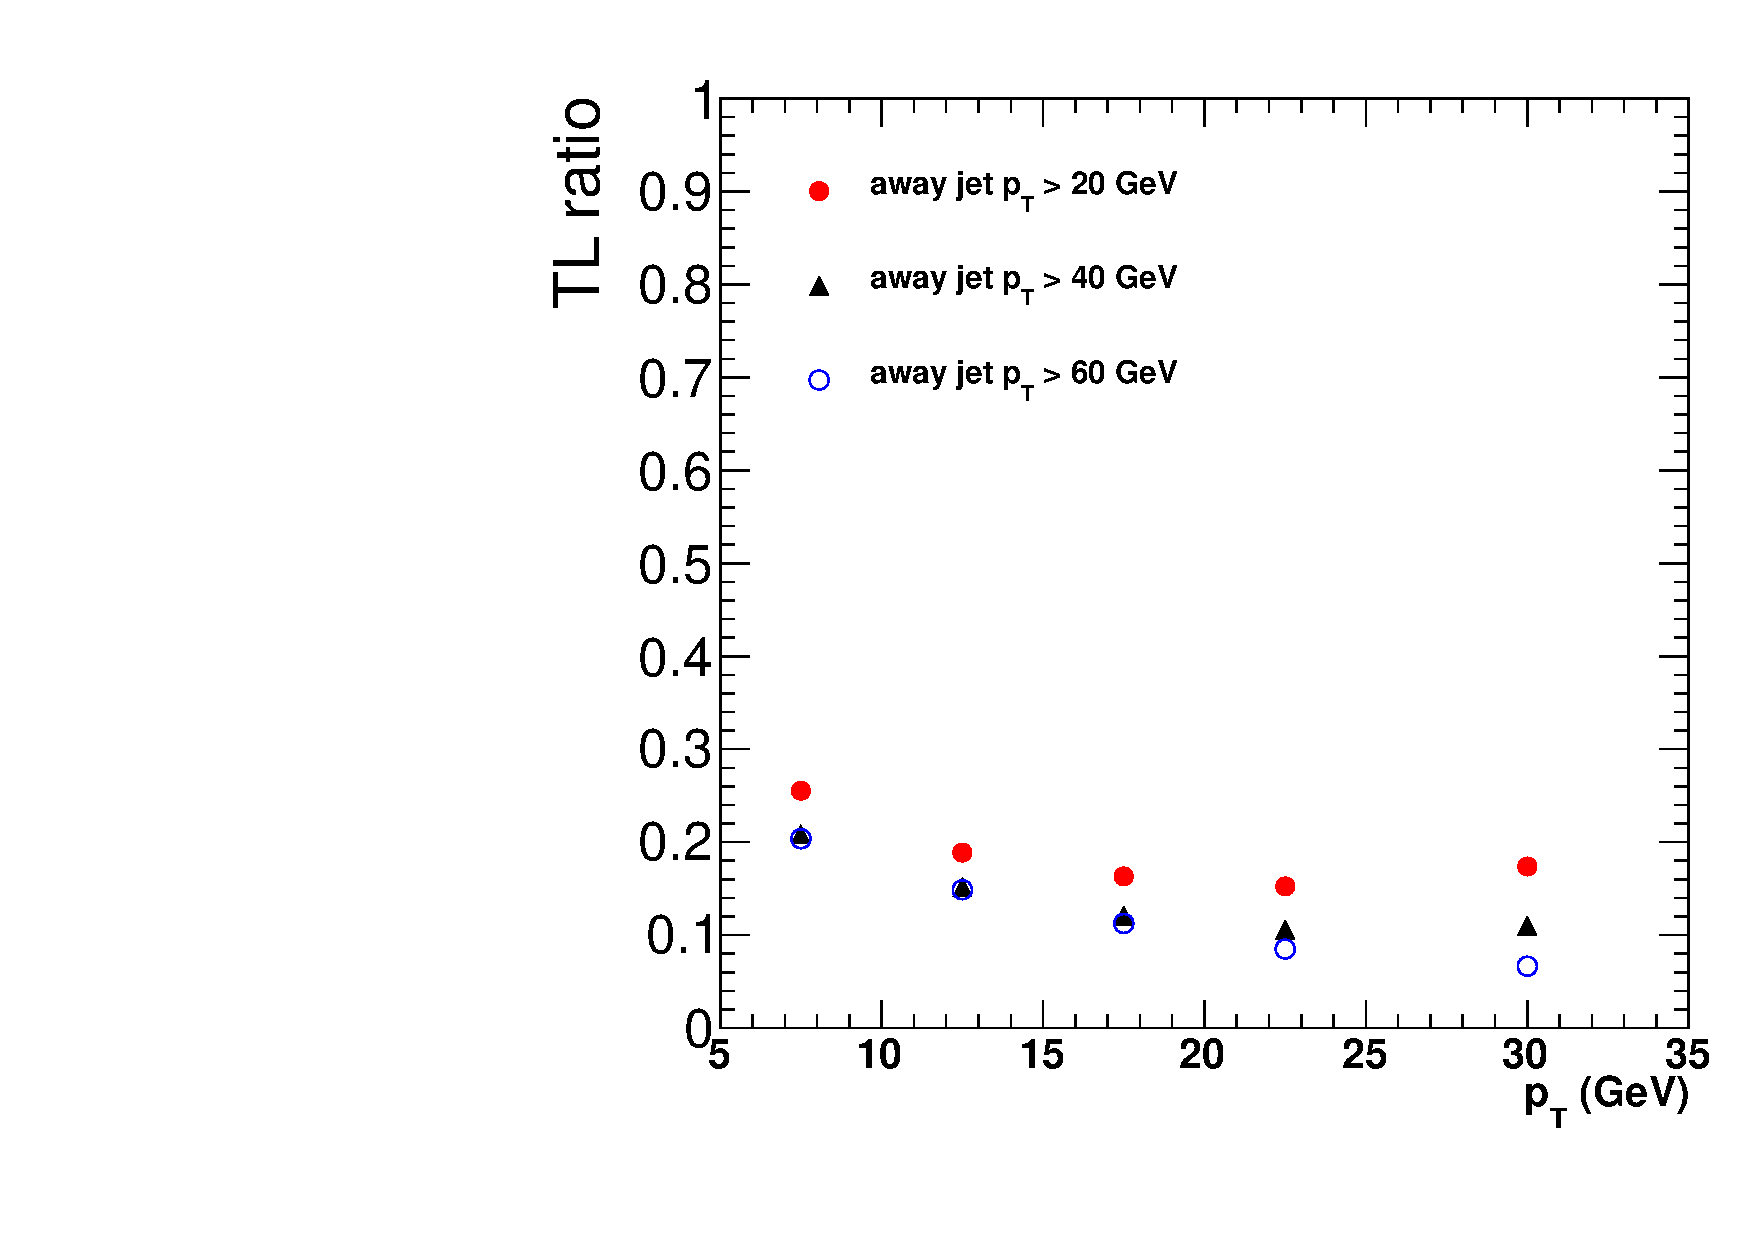
\includegraphics[width=0.48\linewidth]{figs/muFR_data_ptProj}
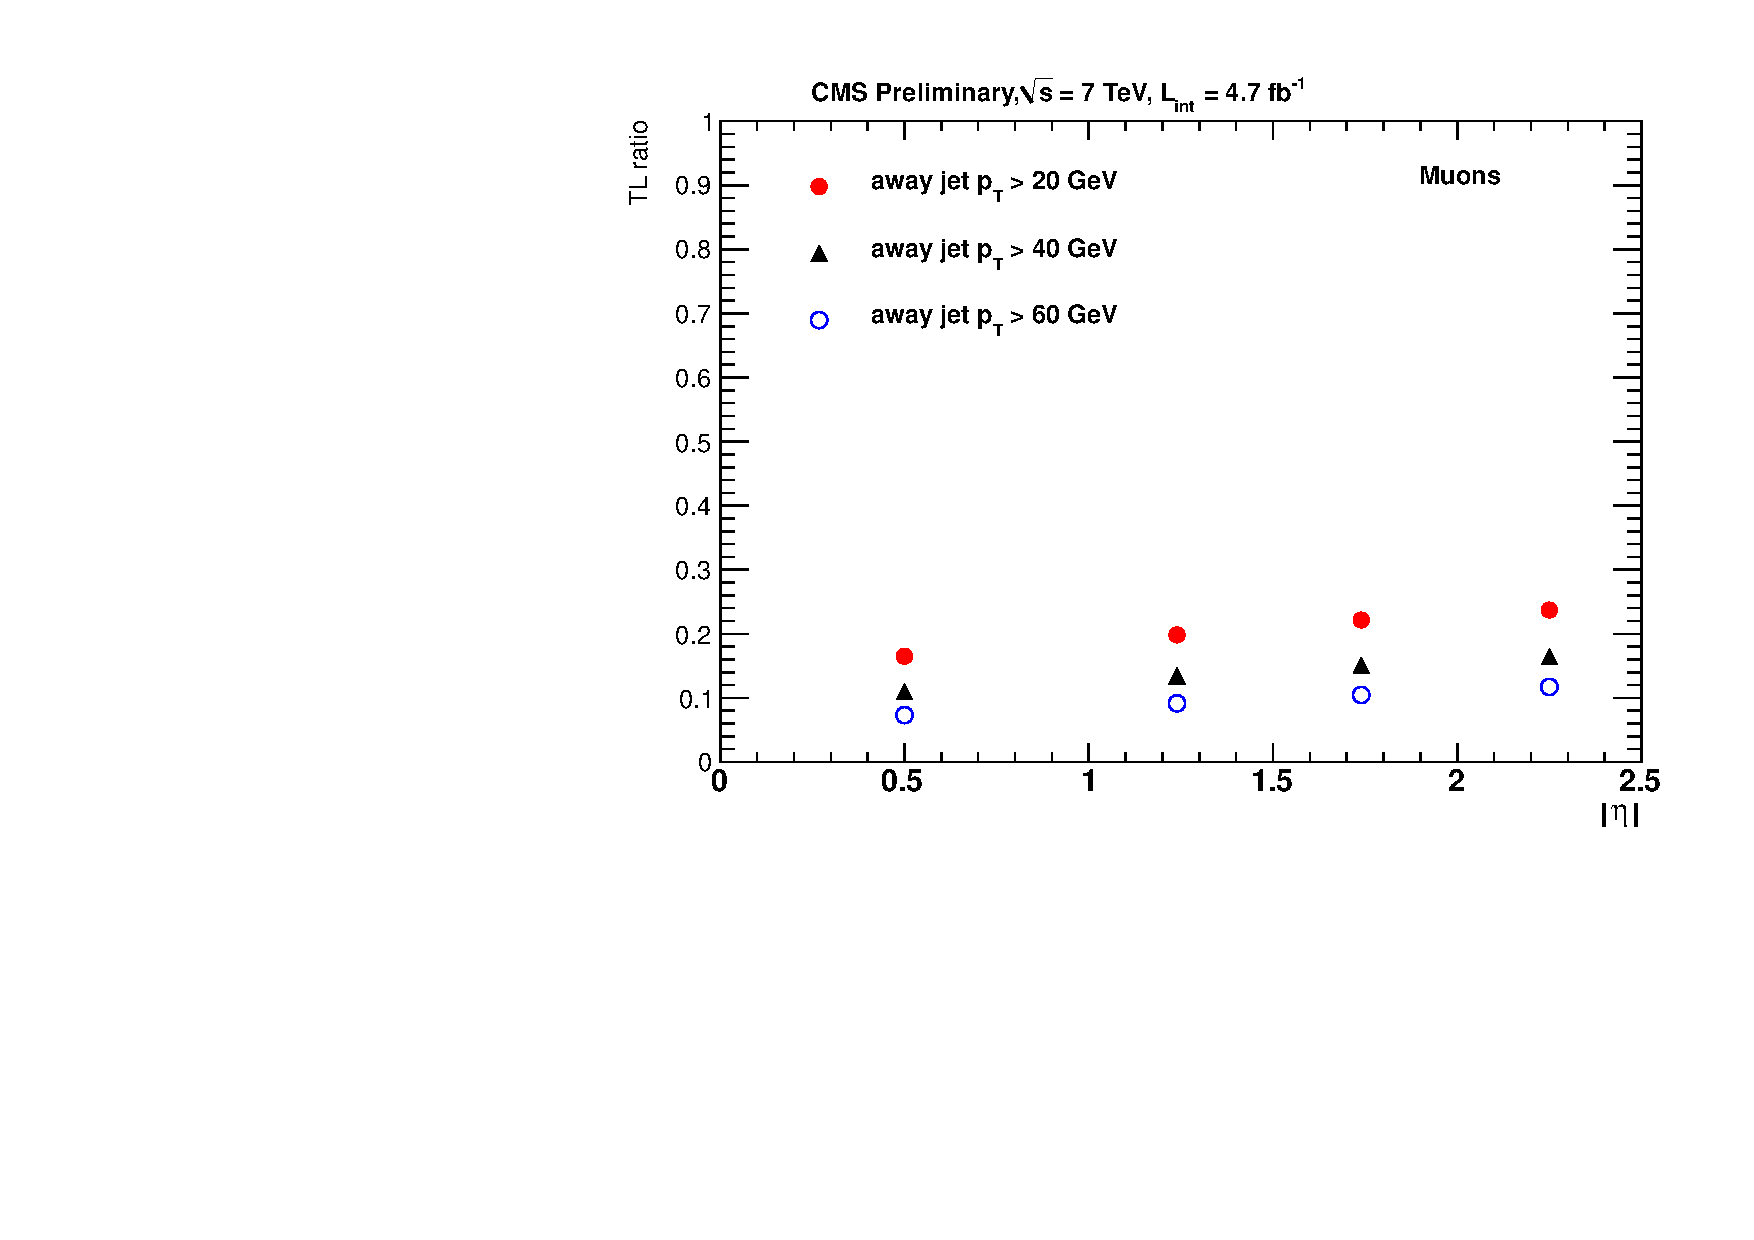
\includegraphics[width=0.48\linewidth]{figs/muFR_data_etaProj}
\caption{\label{fig:frmuon}Muon fake rate projected on $\pt$ (left) and $|\eta|$ (right).
The fake rates are shown separately for measurements  with a requirement for an away jet \pt\ 
to be above 20~\GeV\ (red circles), 40~\GeV\ (black circles), and 60~\GeV\ (blue circles).
}
\end{center}
\end{figure}

\begin{figure}[h]
\begin{center}
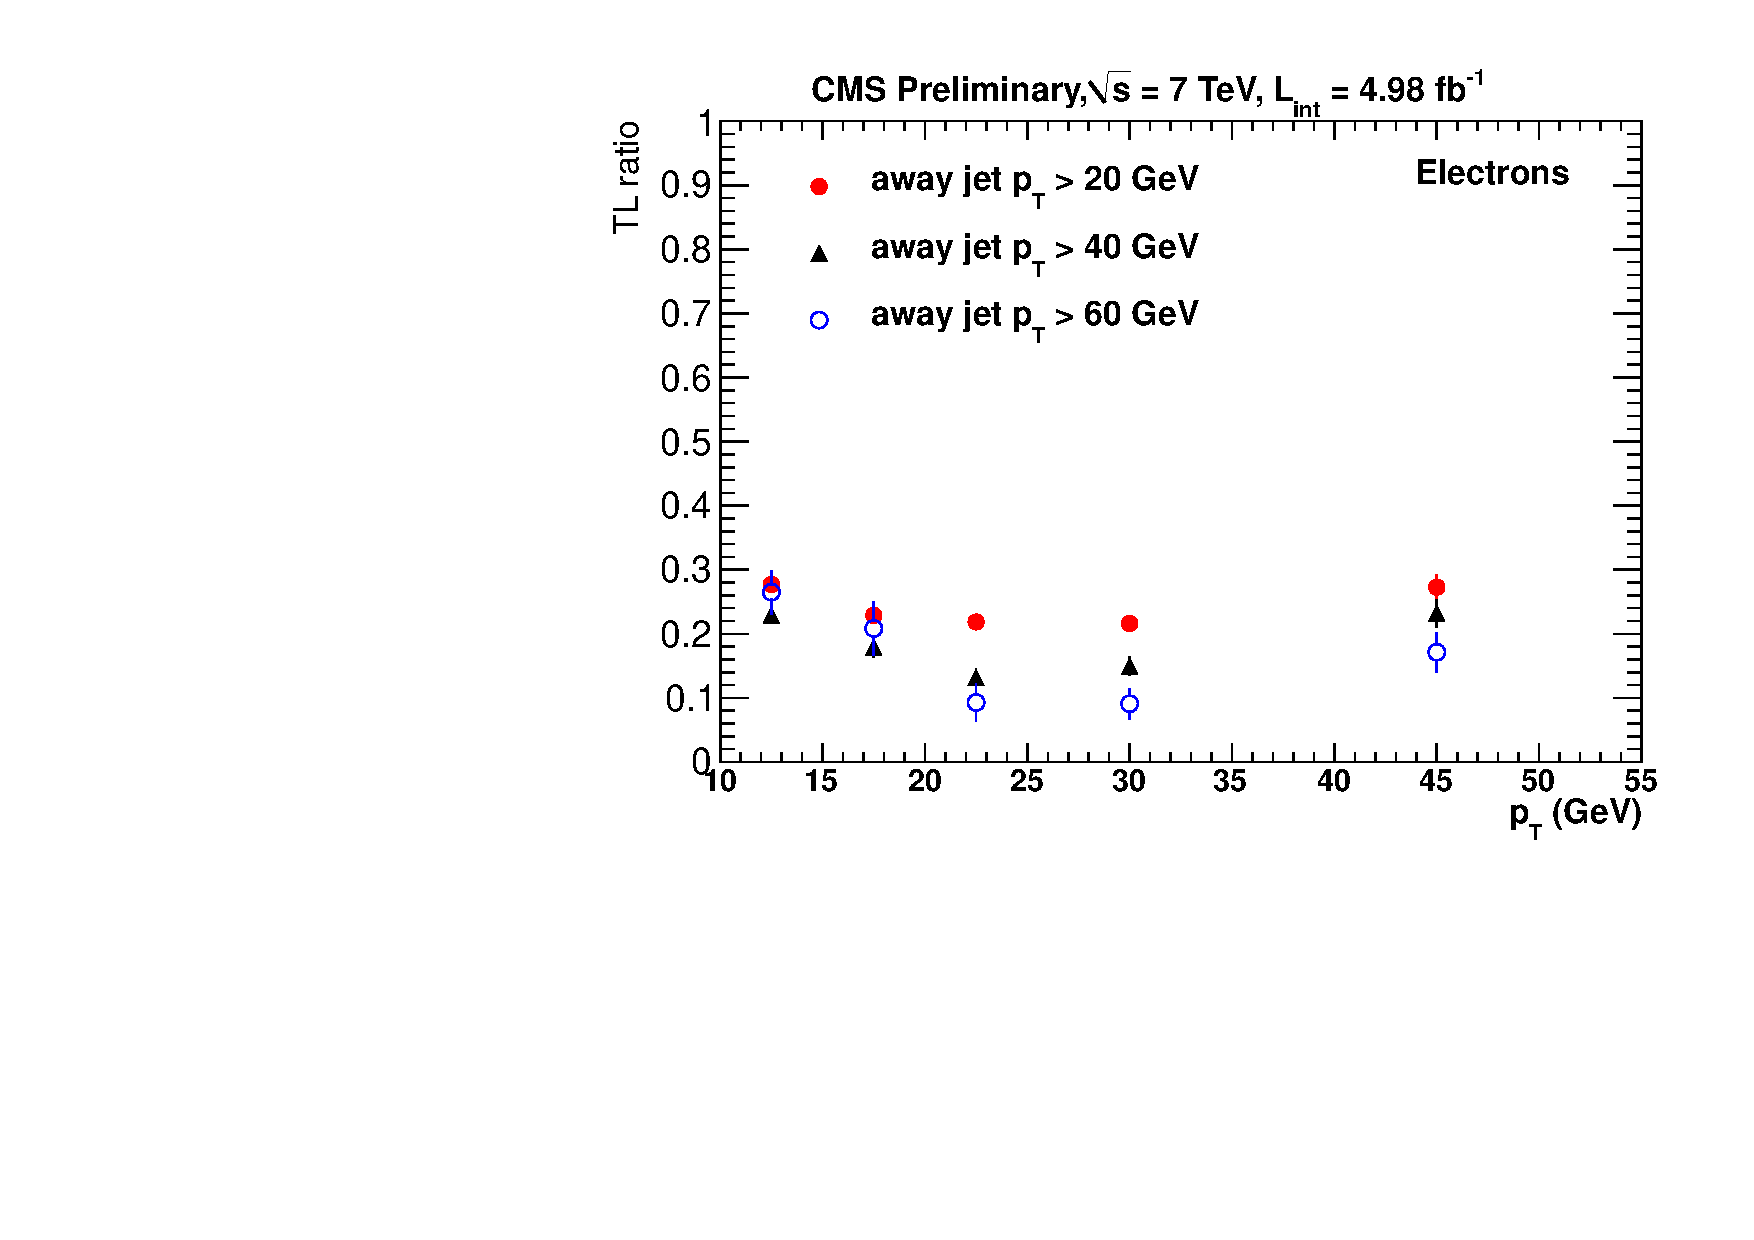
\includegraphics[width=0.48\linewidth]{figs/eleFRcaloIsoTrkIso_data_ptProj}
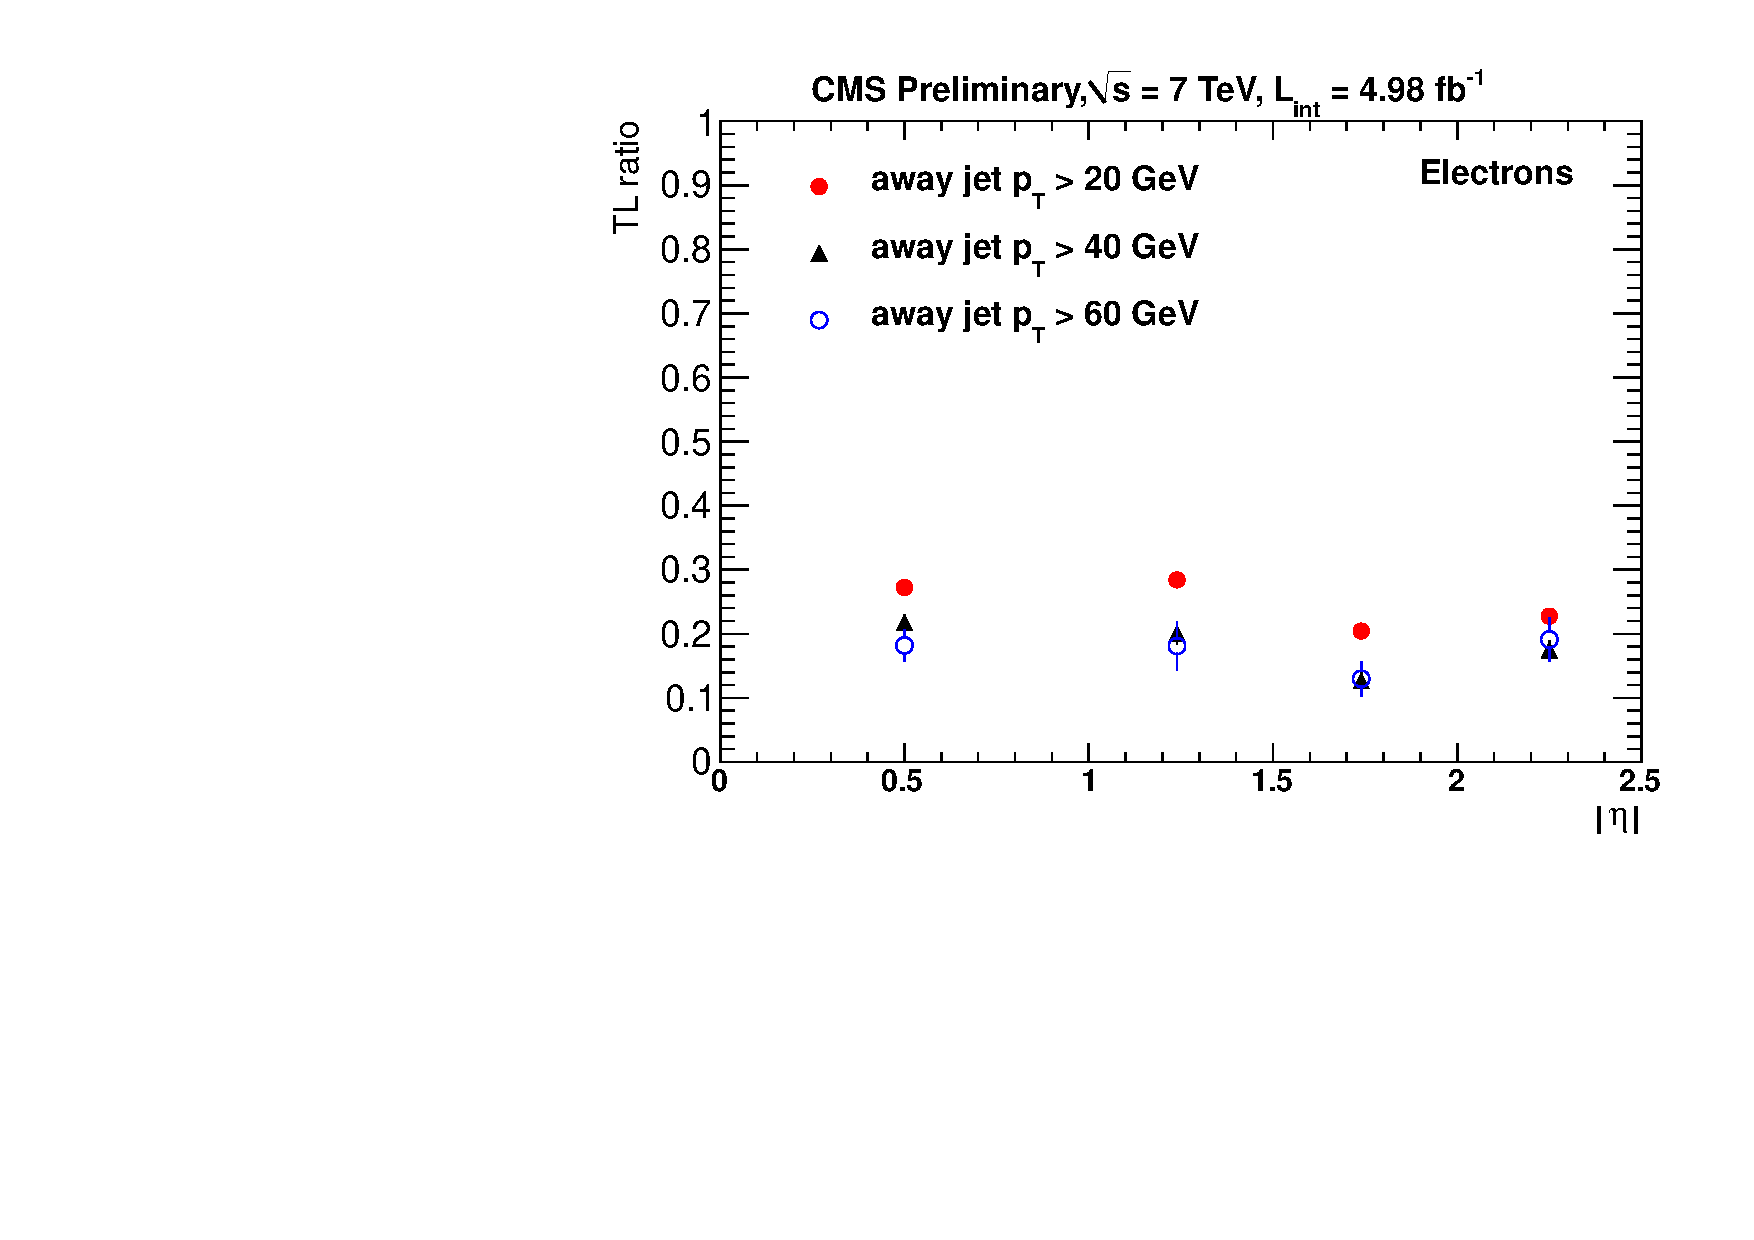
\includegraphics[width=0.48\linewidth]{figs/eleFRcaloIsoTrkIso_data_etaProj}\\
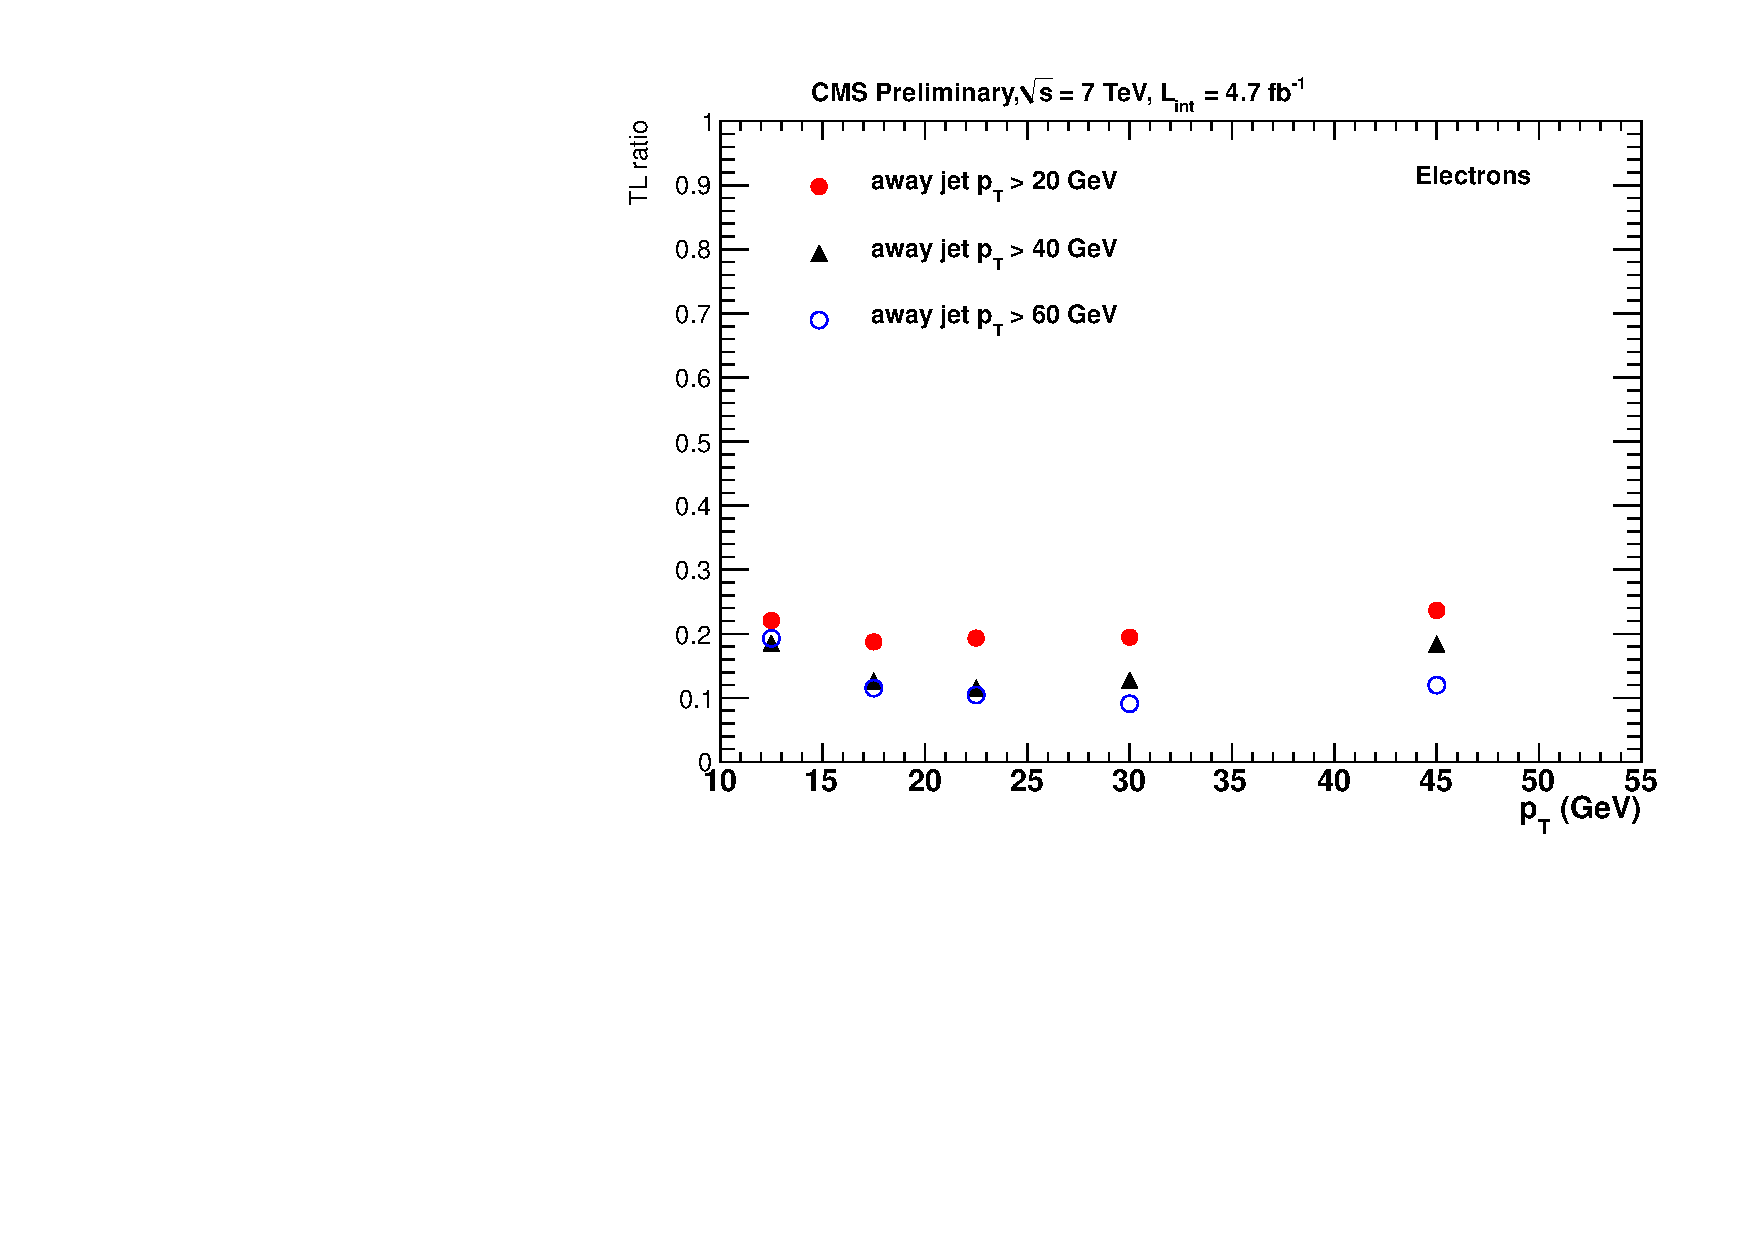
\includegraphics[width=0.48\linewidth]{figs/eleFRcaloIso_data_ptProj}
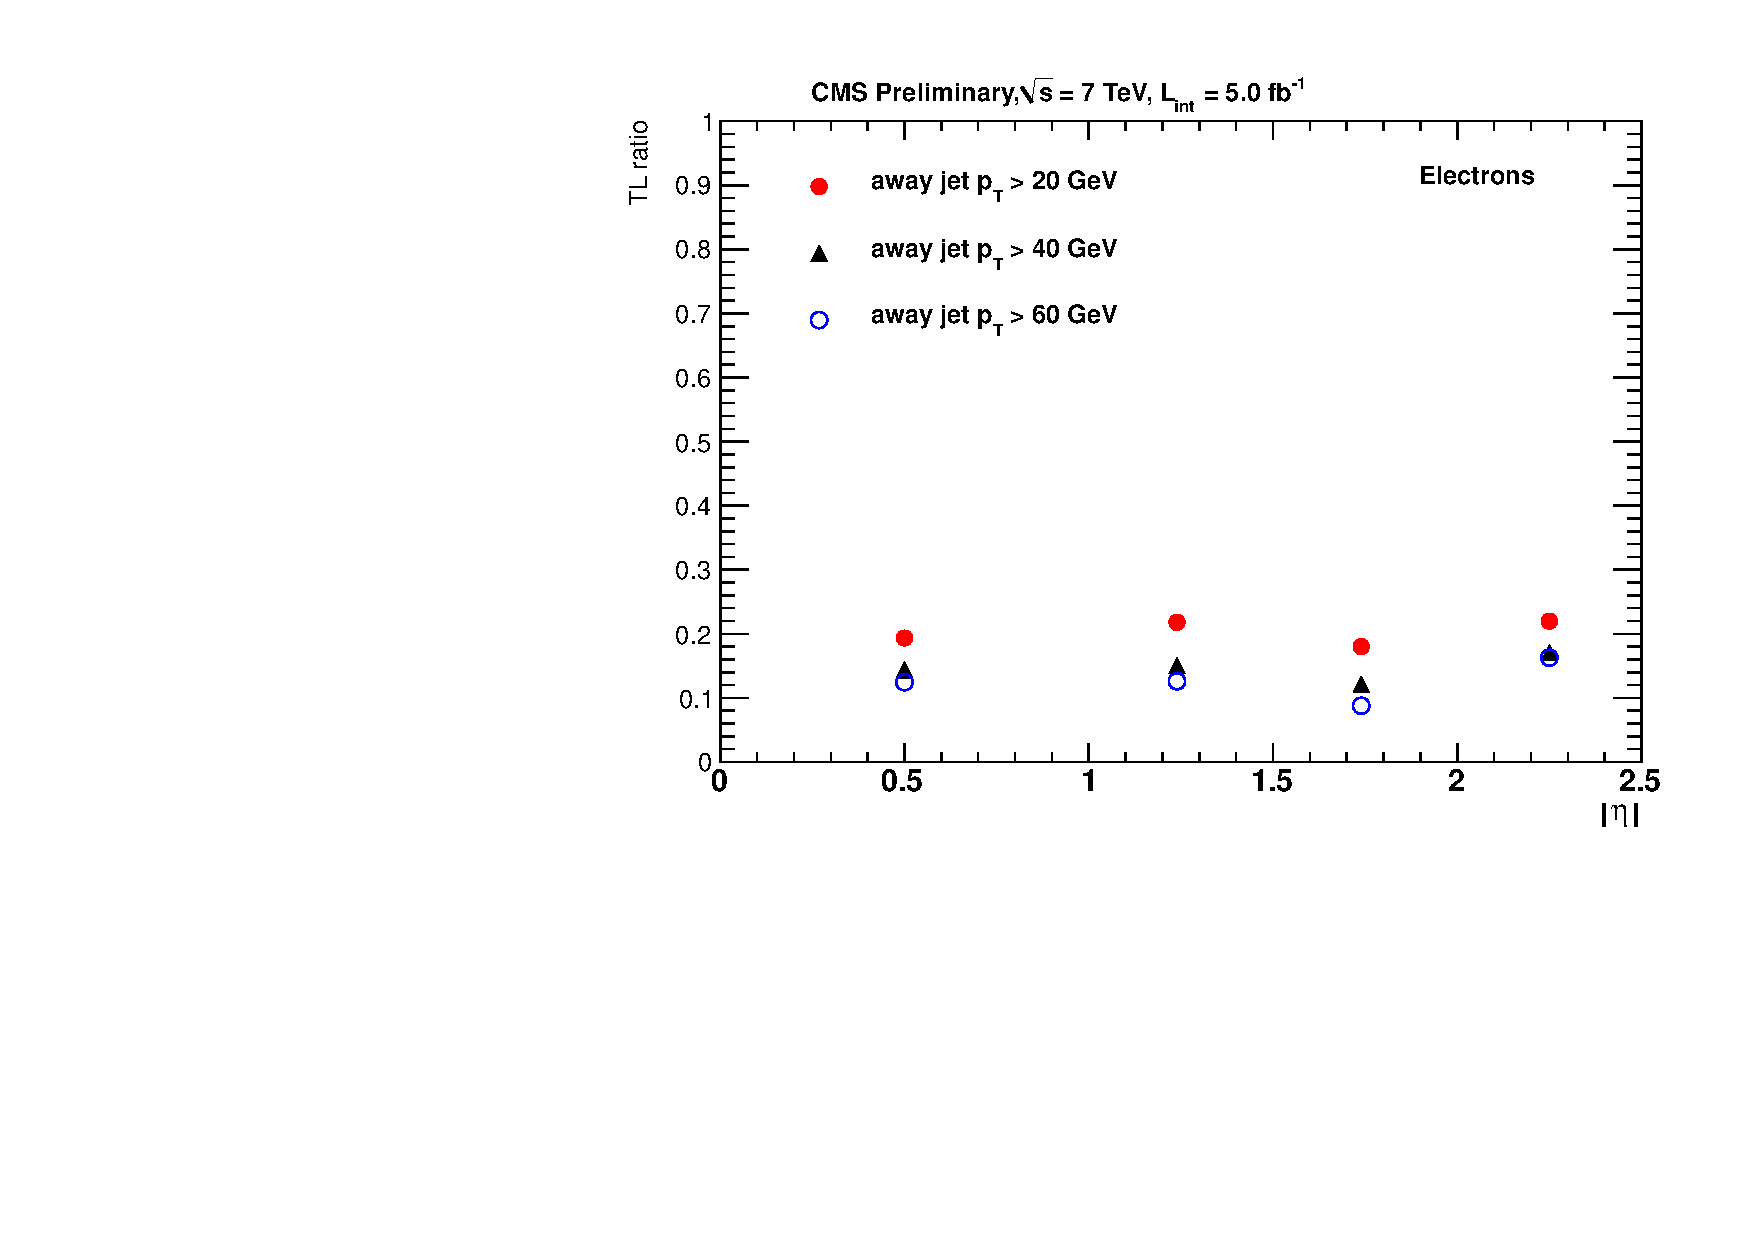
\includegraphics[width=0.48\linewidth]{figs/eleFRcaloIso_data_etaProj}\\
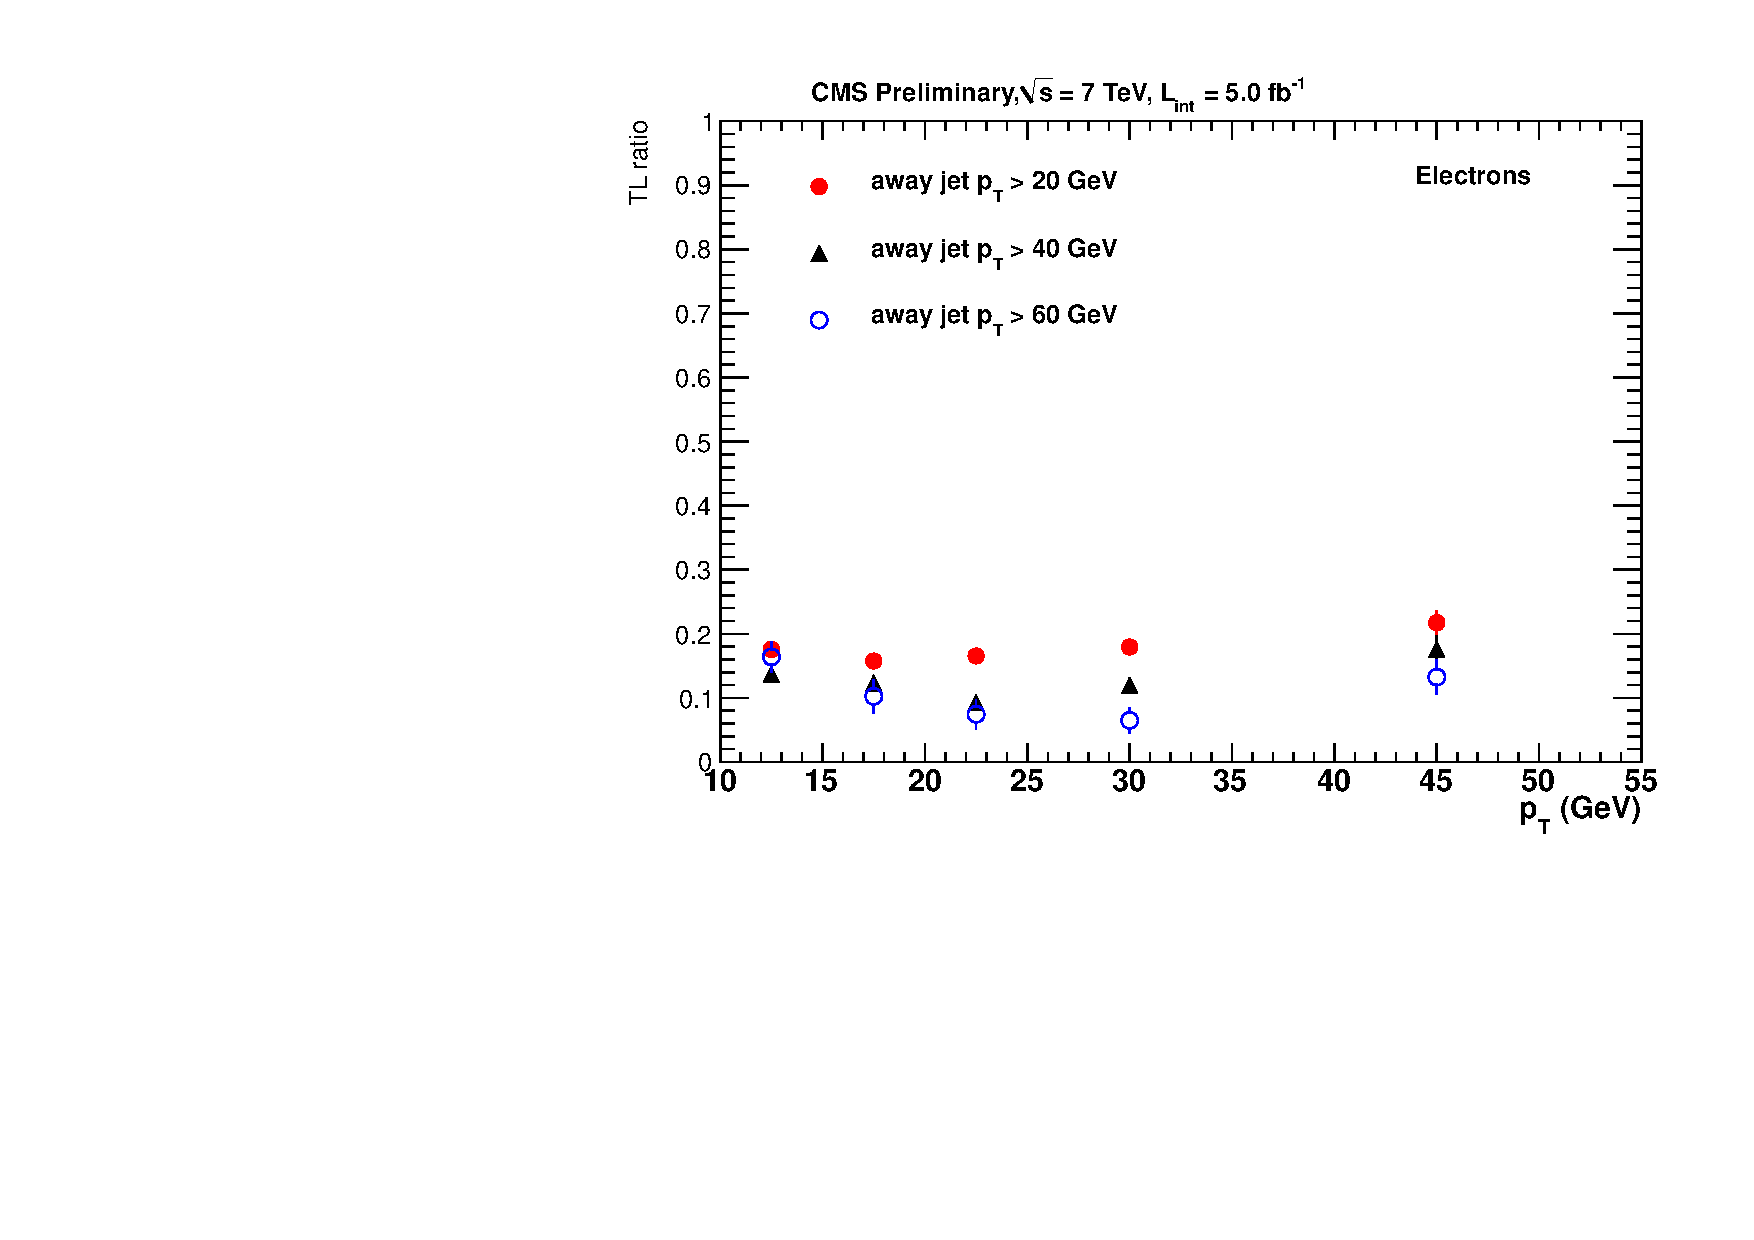
\includegraphics[width=0.48\linewidth]{figs/eleFRnoIso_data_ptProj}
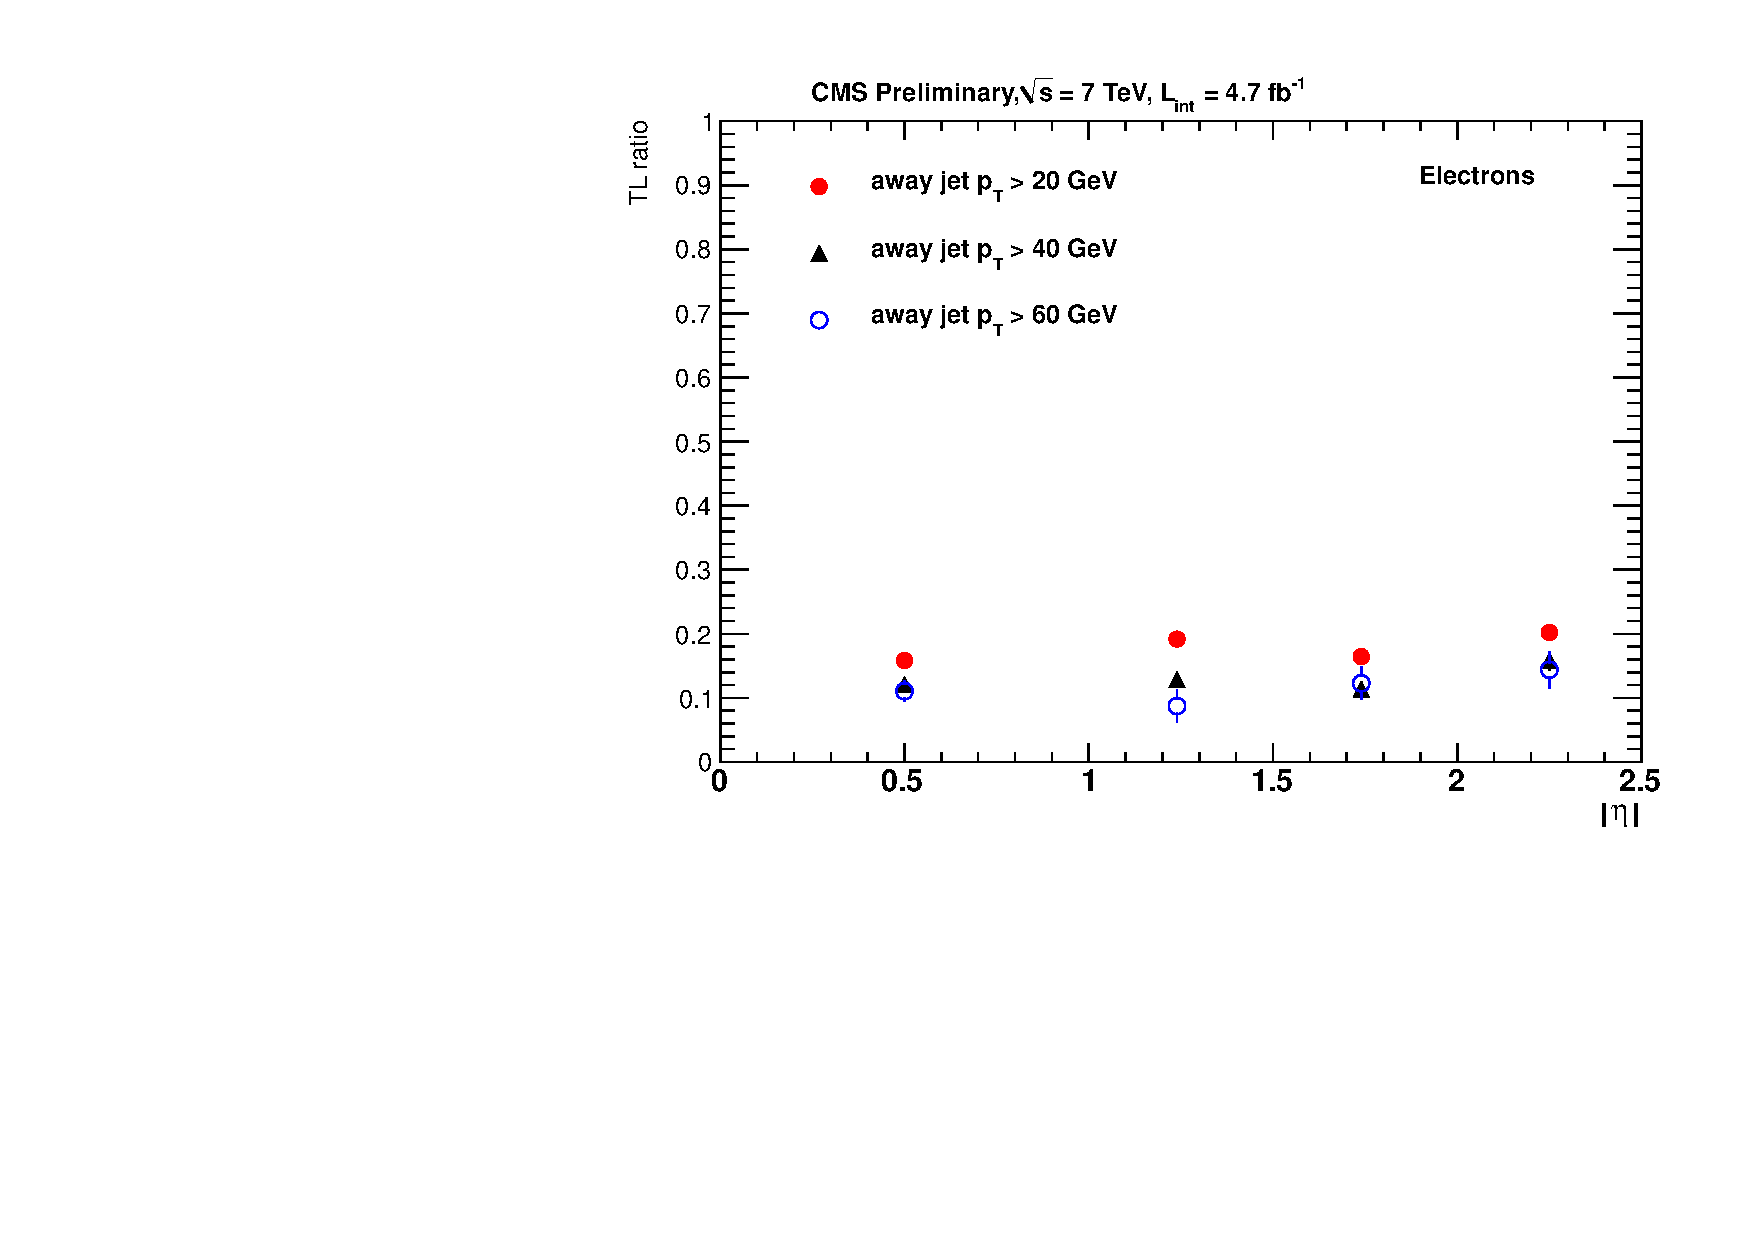
\includegraphics[width=0.48\linewidth]{figs/eleFRnoIso_data_etaProj}
\caption{\label{fig:frelectron}Electron fake rate projected on $\pt$ (left) and $|\eta|$ (right)
for electrons collected by the triggers with calorimeter and tracker isolation requirements (top), 
with a calorimeter isolation requirement (middle) and without an isolation requirement (bottom).
The fake rates are shown separately for measurements  with a requirement for an away jet \pt\ 
to be above 20~\GeV\ (red filled circles), 40~\GeV\ (black up triangles), and 60~\GeV\ (blue open circles).
}
\end{center}
\end{figure}

\clearpage

The application of the fake-rate method to predict this background is exactly the same as in 
the inclusive analysis~\cite{ssnote2011}.
As in the inclusive same-sign analysis, the measured fake rates are restricted to $\pt<55 (35)~\GeV$
for electrons (muons), where we find the contamination from electroweak sources (W/Z production) to be negligible.
The values for the highest measured \pt\ range apply for all leptons with larger momenta.
Measurements for lepton $\pt<20~\GeV$ are given for completeness, they are not used in the analysis.

We test that the fake rates measured in QCD are applicable to the dilepton samples by performing closure
tests on the simulated \ttbar\ sample.\footnote{A large {\tt /TTJets\_TuneZ2\_7TeV-madgraph-tauola/Fall11-PU\_S6\_START42\_V14B-v2} 
sample with an equivalent luminosity of about 0.4 ab$^{-1}$ is used for the closure test.}
Other dilepton processes with fakes, W+jets with one fake and QCD with two fakes, are expected
to contribute negligibly to the events selected in this analysis;
available samples for these processes do not have events passing the baseline selections.
The following selections are applied to events entering the closure tests
\begin{enumerate}
\item select events passing the baseline selections;
\item require that one lepton is matched to a leptonic W decay and the other (fake) lepton is not
matched to a leptonic W decay;
\item scale the number of fake leptons failing the full lepton selections and passing the FO selections
	by $FR/(1-FR)$ as a function of the fake lepton \pt\ and $|\eta|$ --- this is the prediction
	of the number of fakes passing full lepton selections;
\item compare the predicted and observed number of fake leptons.
\end{enumerate}
The prediction of the number of events with fakes,
averaged among modes, gives a reasonable agreement with the observed counts
within the large statistical uncertainties, as summarized in Table~\ref{tab:ttclosure}.
Most of the events are from fake electrons, expecte to contribute about 3/4 of the total.
The events with muon fakes, still expected to be dominated by heavy flavor decays,
are overpredicted, consistent with observations in the pre-tagged analysis~\cite{ssnote2011}.
The events with electron fakes, expected to be dominated by non-heavy-flavor sources,
are on average predicted fairly well, while the agreement fluctuates up/down per-mode.

\begin{table}[h]
\begin{center}
\begin{tabular}{lc|cc|cc}
\hline\hline
Selection	& result	&	\multicolumn{2}{|c}{ElectronFR}		& \multicolumn{2}{|c}{Muon FR}	\\
		&				&	$ee$		& $e\mu$		& $\mu\mu$	& $e\mu$	\\\hline
Baseline	&	observed		& 80			& 42			& 11		& 4		\\
		&predicted			& $45\pm8$		& $75\pm10$		& $19\pm 6$	& $22\pm6$	\\ 
		& $\delta$			& $-0.76\pm 0.37$	& $0.44\pm0.11$		& $0.43\pm0.25$	& $0.81\pm0.11$	\\ 
		& $\langle \delta \rangle$	& \multicolumn{2}{|c}{$-0.01\pm0.14$}		& \multicolumn{2}{|c}{$0.63\pm0.12$} \\
		& $\langle \delta \rangle$	& 		\multicolumn{4}{|c}{$0.15\pm 0.11$}				\\ \hline
\hline
\end{tabular}
\caption{\label{tab:ttclosure}Fake rate closure test on \ttbar\ MC events.
The difference $\delta$ is defined as $(p-o)/p$, where $p$ and $o$ are the predicted
and observed counts, respectively.
The number of events are as counted in the \ttbar\ MC sample.}
\end{center}
\end{table}

\newcommand{\nNoNu}{\ensuremath{N_{{n}\overline{n}}}}
\newcommand{\nNoNo}{\ensuremath{N_{\overline{n}\overline{n}}}}
\newcommand{\nNuNu}{\ensuremath{N_{{n}{n}}}}

The systematic uncertainty of $\pm 50\%$ per fake lepton is estimated for the fake rate method.
This value is dominated by the results of the closure tests.
Our understanding of these results is that the main underlying cause 
the dependence of the fake rate on parent parton momentum.
The momentum spectrum of partons from ISR/FSR differs from that of the b-jets
or light-flavor-quark jets ($W\to q\bar{q}^\prime$) arising from the $t\to W b$ decays.
The mix of the spectra varies, but the range of the fake rate variation
can be tested in data QCD events used to measure the fake rate
by applying varying thresholds to the away jet, as illustrated in Figs.~\ref{fig:frmuon} and~\ref{fig:frelectron}.

We compute the contributions from double-fake and single-fake events separately and assign a 50\% systematic
uncertainty on the combined estimate.

We have neglected any "signal contamination". 
Signal contamination enters when there is a significant
source of two isolated leptons, with one or both failing the numerator cuts, but passing the denominator cuts
comprising  a significant fraction of the total number of \nNoNu\ or \nNoNo\ samples. 
Without an additional correction that can be easily applied,
a contribution from events with two real same-sign dileptons failing the numerator selections
 will overestimate the background contribution by approximately 3\% of the count of
the real same-sign dileptons passing the numerator selections.
Considering the size of the uncertainty on the background,
this effect can be safely ignored in the estimates 
of the fake leptons until the rate of same-sign dileptons passing the full
selections is at least an order of magnitude  higher than that expected
from fakes alone.

%%%%%%%%%%
%%%%%%%%%%

\subsection{Data Driven prediction for charge mis-reconstruction backgrounds}
\label{sec:flips}

%%%%%%%%%%
%%%%%%%%%%

Following our original studies~\cite{sspaper2010} of the electron charge misreconstruction, 
we apply the requirement for electrons that all three charge measurements for a GSF electron agree. 
This dramatically reduces the rate of charge mismeasurement for electrons to the point where it 
is an almost negligible source of background, less than 10\% of the background due to fake leptons~\cite{sspaper2010,ssnote2011,sspaper2011}.
Even though this background is small, it is not necessarily well-reproduced in simulation.
We apply the data-driven method used in the previous analysis here.

The following steps are done:
\begin{enumerate}
	\item Measure the probability for an electron to have its charge misreconstructed 
		in bins of $|\eta |$ and $\pt$ using single electron gun Monte Carlo.
		This is the same probability as measured in the pre-tagged same-sign sample analysis~\cite{ssnote2011}.
	\item Calibrate this probability using Z events in data. 
		This step should be repeated here because of the tighter isolation requirement applied to electrons.
	\begin{enumerate}
		\item Use a Z sample in data to control this probability.
			The sample is selected from dielectron events with $76$\ GeV $ < m_{ll} < 106$\ GeV,  
			\met $ < 20$\ GeV, and transverse mass $< 25$ GeV.
			Here transverse mass is calculated based on whichever lepton has higher $\pt$. 
		\item Apply this probability to the opposite sign events in this control sample
			to obtain a predicted number of same-sign Z candidates.
			Compare this with the actual yield of double-charged Z candidates
			to establish validity of the approach.
		\item If the expected and observed yields agree reasonably well in the previous step, continue using
			the probability measured in the first step and include the discrepancy as a systematic uncertainty.
	\end{enumerate}
	\item Apply this (calibrated) probability to all the electrons in opposite sign dilepton events that pass the selection. 
		This produces the data driven charge flip  prediction shown in the tables in Section~\ref{sec:yields}. 
	\item The $p_T$ distribution of leptons from top is slightly harder than that for leptons from Z. 
		The calibration step above thus does not fully sample the lepton spectrum for our background sample. 
		We assign an additional systematics of 20\% to account for this effect.
\end{enumerate}

In the calibration step we find 390 events with same-sign electron pairs in data in the Z control region.
This needs to be compared with the sum of the expected same-sign events as estimated from
opposite-sign dielectrons, $360\pm4$, plus a contribution from fakes, $11\pm 6$.
These comparisons are consistent within statistics and no additional data-driven correction
is necessary for the simulated charge misid probabilities.
The number of events expected directly from simulation is  $369\pm 11$, also in a good agreement with the numbers above.
The same-sign dielectron mass distribution observed in data is compared to the expectation from
simulation in Fig.~\ref{fig:flipZee}.
The total systematic uncertainty on the charge flip prediction is 20\%,
accounting for both the potential residual miscalibration (less than 5\%) and the difference in the lepton
spectra in Drell-Yan events and in the background \ttbar\ events.


\begin{figure}[h]
\begin{center}
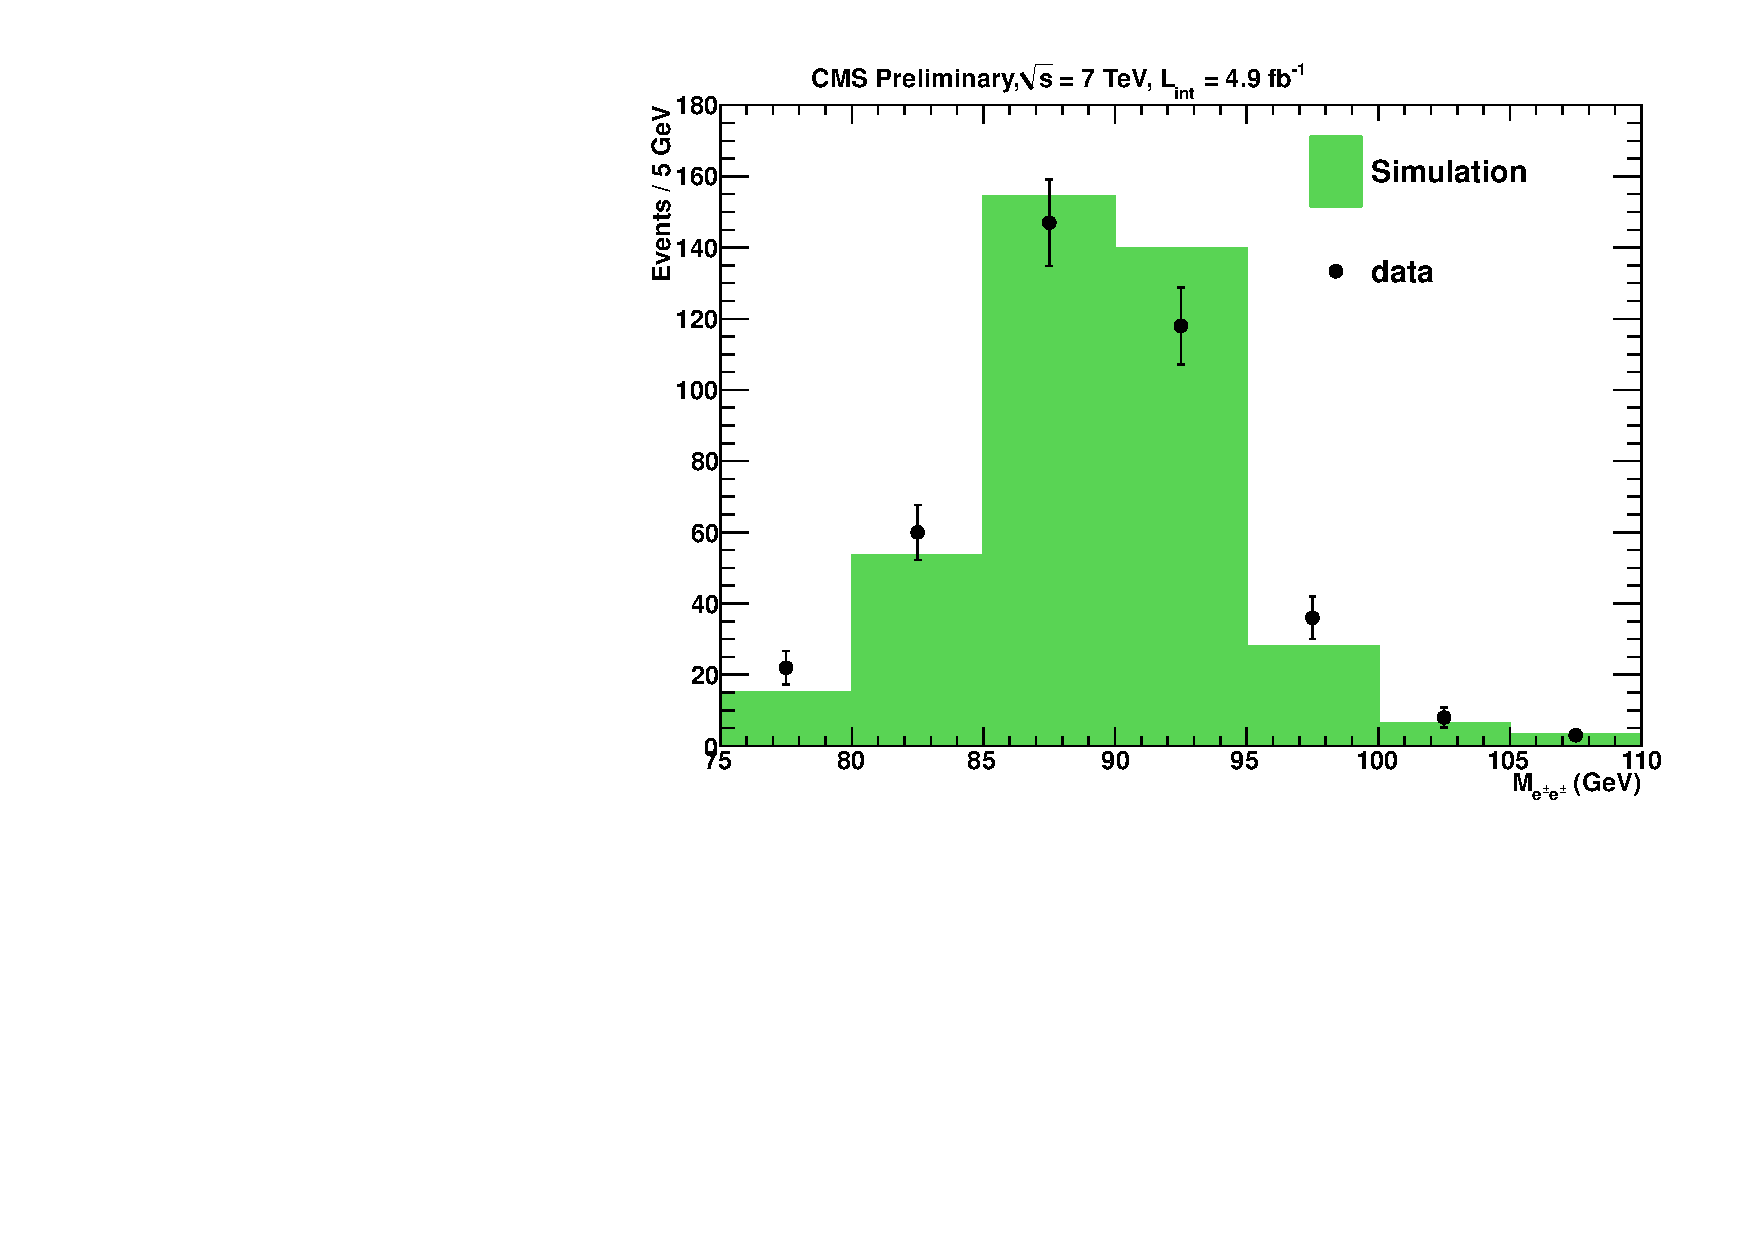
\includegraphics[width=0.8\linewidth]{figs/qflip_data_mc_comp}
\caption{\label{fig:flipZee}
Same sign $ee$ invariant mass distribution compared with $Z \to ee$ Monte Carlo expectations.
Cuts on missing transverse energy $<$ 20 GeV and transverse mass
$<$ 25 GeV have been applied to reduce backgrounds from $W +$ jets.
The highest $\pt$ lepton has been used in the calculation of the transverse  mass.}
\end{center}
\end{figure}


